%!TEX root = ../thesis.tex

\section{Server Infrastructure}
\label{sec:server_infrastructure}

The smart heating server is the central storage and communication center of this project.
It persists data collected by the local deployment as also organizational information and heating schedules provided by the user via the Mobile App.

\subsection{Design Goals}
\label{sec:server_infrastructure_design_goals}

\begin{itemize}
\item \emph{Modularity} for independent, interchangeable components for improved maintainability.
\item \emph{Extensibility} to easily add new resources and relationships.
\item \emph{Usability} to allow developers simple inspection of the API structure and modification of resources.
\item \emph{Testability} for good and comprehensible tests and high software quality.
\end{itemize}

\subsection{Platform and Frameworks}
\label{sec:server_infrastructure_platform_and_frameworks}

The server is implemented with Python, a general-purpose, multi-paradigm programming language\footnote{\url{https://www.python.org/}}.
Python was chosen as it is suitable for developing a solid web server as well as the embedded hardware used for the communication gateway in the local deployment. See Section~\ref{sec:local_infrastructure} for more explanation.
Django is a popular, open-source web application framework\footnote{\url{https://www.djangoproject.com/}} based on a model-view-controller (MVC) pattern facilitating the development of complex, database-driven web applications.
The Django REST Framework\footnote{\url{http://www.django-rest-framework.org/}} extends Django to support the design of RESTful\footnote{Note: REST is a programming paradigm where as RESTful is used to describe a web application implementing such a paradigm.} Web APIs.

\subsection{RESTful API}
\label{sec:server_infrastructure_restful_api}

The smart heating server provides a RESTful API to access a persistent storage providing the basic CRUD operations: Create, Read, Update and Delete.
Representational State Transfer (REST) is a programming paradigm used for machine-to-machine communication in distributed systems.
RESTful web services use HTTP as their preferred communication protocol.

REST is about resources.
Each resource is identified by a uniform resource identifier (URI) and is accessible via the request methods defined in HTTP.
We differentiate two major types of URIs: Resource collections and resource representations.
A resource representation is a view of its resource's state and is encoded in a transferable format.
This project uses the simple JavaScript Object Notation (JSON) format to represent resources.
Resource collections contain lists of representations of the same type of a resource.

\paragraph{Design Decisions}

\begin{enumerate}
    \itemsep0em
    \item The underlying model hierarchy is represented via nested URLs.
    \label{enum:design_decision_nested_urls}
    
    \item The resource identifier is the first field in each resource representation.
    \label{enum:design_decision_identifier_first_field}
    
    \item Within resource representations, collections are referenced via URL. Resources are referenced by including their representation.
    \label{enum:design_decision_resource_referencing}
    
    \item URL fields are identified by the name \highlight{url} or the suffix \highlight{\_url}. Each resource representation contains its own URL in the field \highlight{url}.
    \label{enum:design_decision_url_fields_prefix}
\end{enumerate}

See Listing~\ref{lst:room-json-example} for an example of a resource representation.

\begin{snippet}[language=JavaScript,label={lst:room-json-example},caption={Example representation of the Room resource at \nolinkurl{http://server/residence/04891BB9232584/room/2/}.
		The \highlight{url} field determines the URL of the represented resource.
		Within the \highlight{residence} field the representation of the associated Residence resource is nested.
		The included Residence representation has its own \highlight{url} field.
		Collections of the Residence's Rooms and Users are not nested but referenced via URL to limit the response size.}]
	{
		"id": 2,
		"url": "http://server/residence/04891BB9232584/room/2/",
		"name": "Dining Room",
		"residence": {
			"rfid": "04891BB9232584",
			"url": "http://server/residence/04891BB9232584/",
			"rooms_url": "http://server/residence/04891BB9232584/room/",
			"users_url": "http://server/residence/04891BB9232584/user/"
		},
		"thermostats_url": "http://server/residence/04891BB9232584/room/2/thermostat/"
	}
\end{snippet}


\paragraph{Browsable API}

The Django REST Framework offers the ability to dynamically generate a browsable interface accessible via web browser.
It includes a formatted output of the JSON response, offers forms to add new resources and edit or delete existing resources, and displays URLs as clickable hyperlinks.
This interface is an additional HTML output format enabling developers to easily interact with the API without the need of external tools.
The Browsable Web API is designed for readability whereas the API renders its data as compressed JSON to reduce transmission bandwidth. \todo[inline]{MICHAEL: "bandwith" - Can't think of the correct word..}
See Figure~\ref{fig:server_infrastructure_browsable_api} for an example.

\begin{figure}[h]
	\begin{center}
		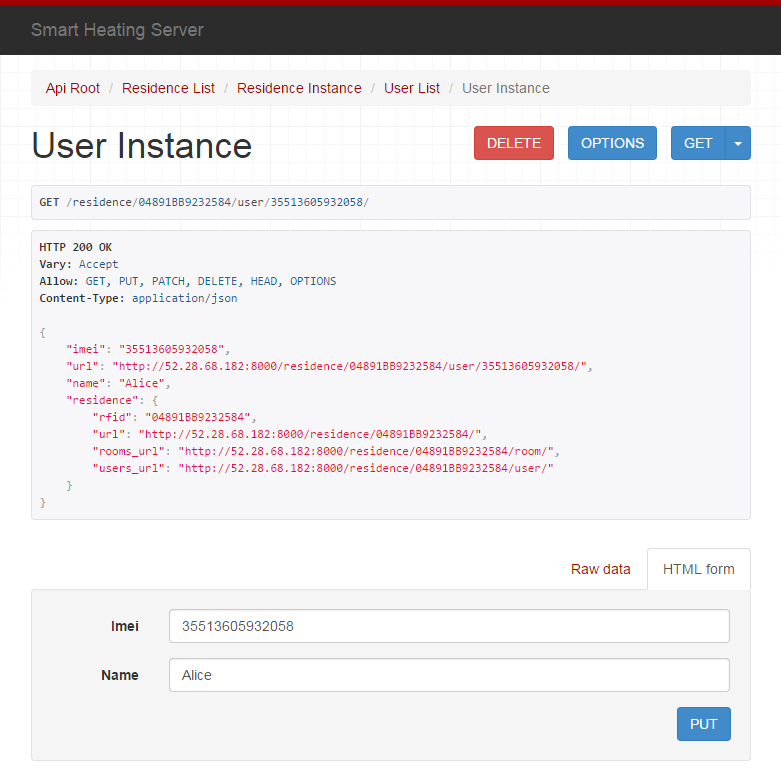
\includegraphics[width=0.8\textwidth]{images/server_browable_api_user_instance.png}
	\end{center}
	\caption{Screenshot of the Browsable Web API showing an instance of a user resource. The interface allows the developer to easily edit or delete the user. Navigating the residence or the associated room or user collections can be done by clicking on the URLs of the respective resources.}
	\label{fig:server_infrastructure_browsable_api}
\end{figure}


\subsection{Program Architecture and Implementation}
\label{sec:server_infrastructure_program_architecture_implementation}

The server implementation is built on Django following a variation
%\footnote{For the interested reader: \url{https://docs.djangoproject.com/en/1.8/faq/general/\#django-appears-to-be-a-mvc-framework-but-you-call-the-controller-the-view-and-the-view-the-template-how-come-you-don-t-use-the-standard-names}}
of the Model-View-Controller (MVC) architectural pattern.
We assume the reader to be familiar with the common MVC pattern\footnote{We refer the interested reader to \url{https://en.wikipedia.org/wiki/Model-view-controller}}.

All the code required to setup the smart heating server is provided in the GitHub repository located at \url{https://github.com/spiegelm/smart-heating-server}.
We highly encourage the reader to visit the project on GitHub.
The main page of the repository provides a short explanation and also contains a hyperlinked image indicating the status of the latest build run on the continuous integration service as explained later in Section~\ref{sec:server_infrastructure_testing}.
The repository is designed to contain all code and dependency information necessary to automatically install and run the application on a server.

The following sections describe the relevant application components in detail.
% TODO explaint the directory structure, project consisting of several apps, namespaces, etc?
%The code repository contains three directories. The first one, \highlight{project}

\subsubsection{Models}
\label{sec:server_infrastructure_models}

Models structure the underlying data and provide operations for manipulating it.
In Django models contain the business logic and are also responsible for validating user input and providing appropriate error messages.
The \highlight{smart\_heating.models} namespace contains all project models.
Each model extends the abstract \highlight{Model} class, providing a general method used to get an objects representation for debugging purposes as well as the abstract \highlight{get\_recursive\_pks} method.
This method is used to generate hierarchical URLs and will be further described in Section~\ref{sec:server_infrastructure_serializers}
% A high level description of all used models is given in Section~\ref{sec:system_overview_models}. 

Thermostats are organized within rooms and belong to a residence.
RaspberryDevice and ThermostatDevice represent the deployed physical devices.
Both are used as a global configuration of all devices that are planned to be eventually installed in a residence.
This configuration associates a device's MAC address to the number of the radio-frequency identification (RFID) tag attached on the device.
This is required to relate these two identifiers, as the hardware cannot read the RFID tag number from the device casing and the mobile application cannot access the internal MAC address used by the devices.
Storing this mapping on the server benefits the deployment of the local devices as every device can use the same code and no configuration of the devices is required.
See Figure~\ref{fig:class_diagram} for a graphical representation of the used models.
The most important models will be described in the following paragraphs.

\begin{figure}[h]
\begin{center}
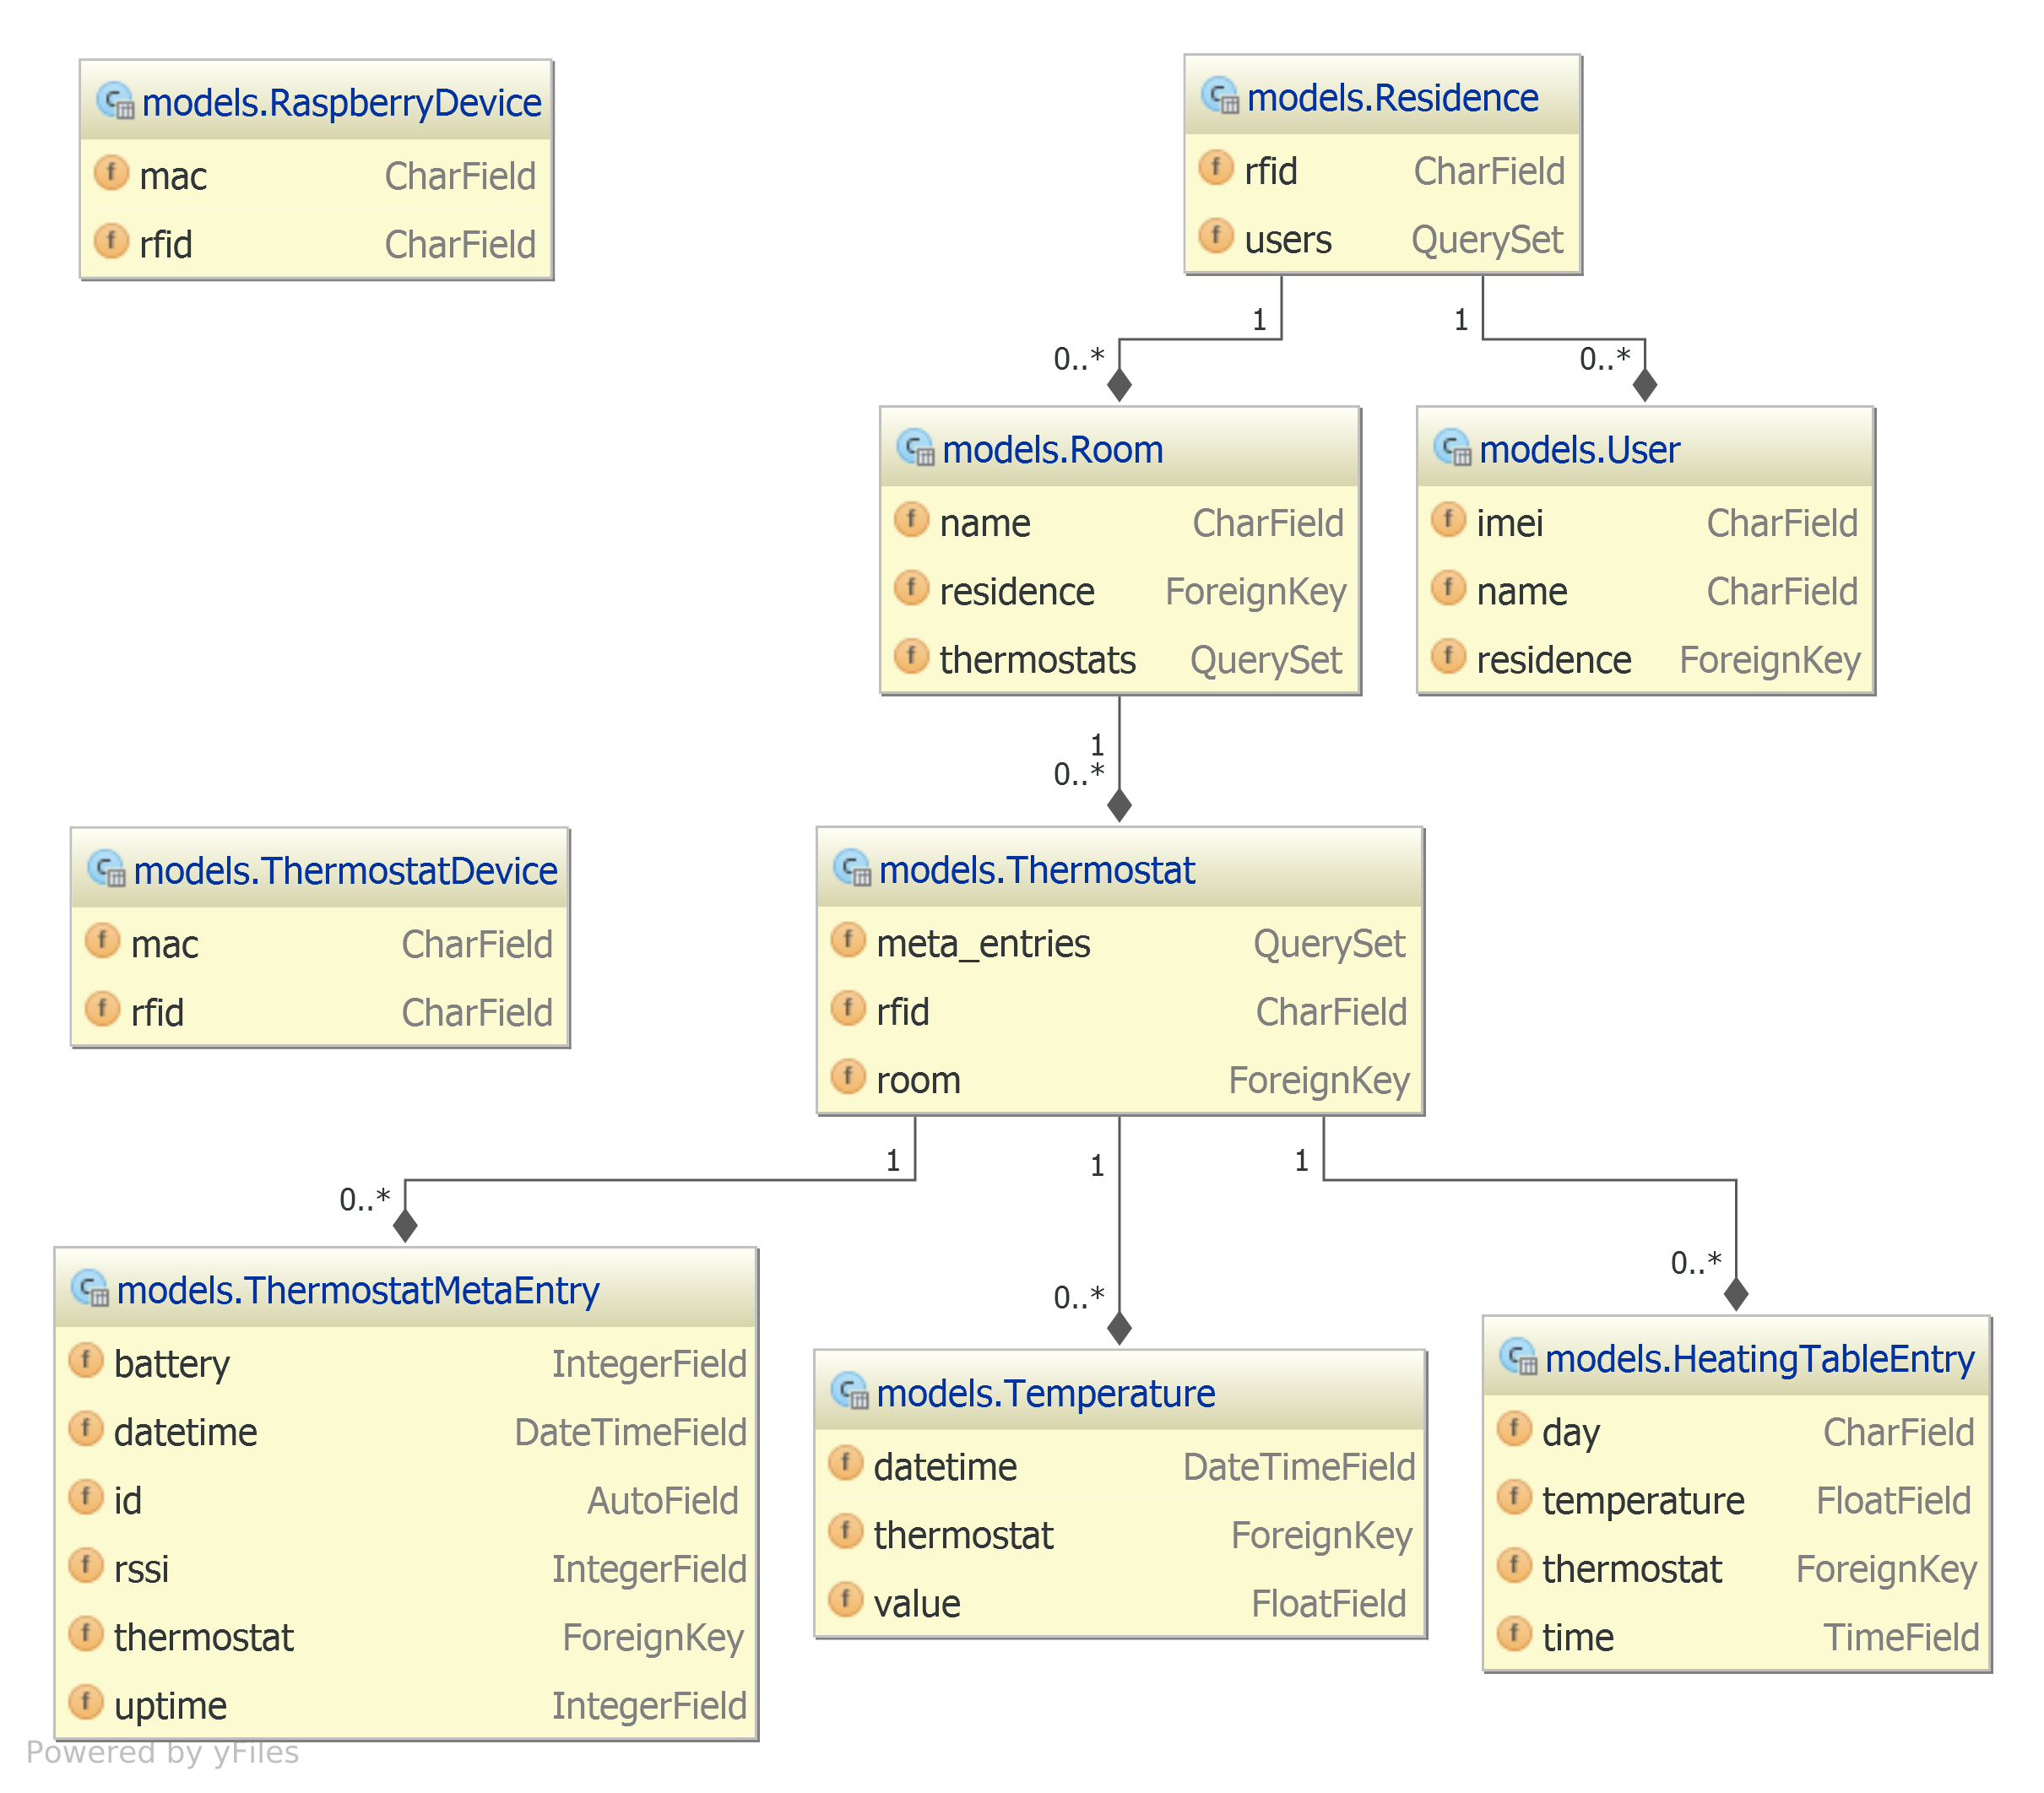
\includegraphics[width=0.8\textwidth]{images/uml_class_diagram_pycharm_highres.png}
\end{center}
\caption{UML class diagram of the used models.
	% TODO
	%\todo[inline]{Fix diagram: add all or remove all Querysets. Decide whether or not to display unique constraints.}
	}
\label{fig:class_diagram}
\end{figure}

\paragraph{Residence} is identified by the RFID tag number on the deployed local communication gateway.
A residence combines users and rooms with their associated thermostats and data into a single encapsulated unit.

\paragraph{User} is identified by the smart phone's serial number\footnote{The International Mobile Equipment Identity (IMEI) is a 15-digit serial number associated to each GSM cell phone.} and can be registered to at most one residence.

\paragraph{Room} groups thermostats into an organizational unit.
Each residence can contain multiple rooms.

\paragraph{Thermostat} is identified by the number of the attached RFID tag.
It is the parent of the models used for the historic temperature and thermostat meta data and the heating schedule.

\paragraph{Temperature} represents a single temperature measurement perceived by a thermostat at a specific date and time.

\paragraph{ThermostatMetaEntry} is used to combine meta data that is available by the digital thermostat such as battery level, system uptime and received signal strength indication (RSSI).

\paragraph{HeatingTableEntry} is used to compose the heating schedule for a thermostat.
An entry determines the target temperature that applies starting from the given day and time until the next heating table entry occurs.

\subsubsection{Serializers}
\label{sec:server_infrastructure_serializers}

Serializers are responsible for translating models into a resource representation and vice versa.
This project uses JSON to represent resources.
Each serializer has an associated model and determines which model fields should be included into the resource representation.
Additional fields can be added to the representation or individual field representations can be overwritten to offer customized output.

A commonly used customization is the replacement of the default \highlight{Hyperlinked\allowbreak IdentityField} with \highlight{Hierarchical\allowbreak Hyperlinked\allowbreak IdentityField}.
This custom serializer field generates URLs according to the hierarchical schema applied in this project.
For example the URL for a room would be \nolinkurl{http://server.com/residence/041FB2B9232580/room/5/}.
To assemble this URL the identifier of the room and its parent are required.
The adapted field extends the default field and provides all identifiers of the hierarchy required to generate the URL by using the hierarchical base class \highlight{smart\_heating.models.Model}.

Nested resources are implemented using nested serializers.
This way existing serializers can be reused to include their resource representation into another representation. Refer to line 3 in Listing~\ref{lst:server_infrastructure_nested_serializer} for an example usage of a nested serializer.

\begin{lstlisting}[label={lst:server_infrastructure_nested_serializer},language={Python},
caption={The \highlight{RoomSerializer} class as an example of the usage of the \highlight{Hierarchical\allowbreak Hyperlinked\allowbreak IdentityField} and nested serializers.
}]
class RoomSerializer(serializers.HyperlinkedModelSerializer):
	url = relations.HierarchicalHyperlinkedIdentityField(view_name='room-detail', read_only=True)
	residence = ResidenceSerializer(read_only=True)
	thermostats_url = relations.HierarchicalHyperlinkedIdentityField(source='thermostats', view_name='thermostat-list',
	read_only=True)
	
	class Meta:
		model = Room
		fields = ('id', 'url', 'name', 'residence', 'thermostats_url')
\end{lstlisting}

\subsubsection{Views}
\label{sec:server_infrastructure_views}

A view is a class which processes requests and returns a response.
Django defines the view as the place that not only defines how but also which data is presented.
This slightly differs from the traditional MVC architectural pattern but will not be explained in detail here\footnote{For more details we refer the reader to \url{https://docs.djangoproject.com/en/1.8/faq/general/\#django-appears-to-be-a-mvc-framework-but-you-call-the-controller-the-view-and-the-view-the-template-how-come-you-don-t-use-the-standard-names}}.
Django includes generic view classes and mixins to provide common functionality and to facilitate code reuse.
The Django REST Framework further abstracts views by supplying \highlight{ViewSets}.
These \highlight{ViewSets} facilitate the unified handling of different HTTP methods within a single class for each public resource.

The used \highlight{ModelViewSet} is such a class serving as a base for individual view sets representing a resource.
In the very simplest case only the definition of a database query and an appropriate serializer class is required.
The \highlight{ResidenceViewSet} is a good example of a fully functional resource implementation supporting all CRUD methods while only requiring three lines of code, as shown in Listing~\ref{lst:server_infrastructure_view_residenceViewSet}.

\begin{lstlisting}[label={lst:server_infrastructure_view_residenceViewSet},language={Python},
caption={The \highlight{ResidenceViewSet} class.
}]
class ResidenceViewSet(viewsets.ModelViewSet):
	queryset = Residence.objects.all()
	serializer_class = ResidenceSerializer
\end{lstlisting}


\paragraph{Pagination} is the practice of partitioning lists into smaller pieces.
In this project pagination is used for expectedly large resource collections such as temperatures or meta entries.
The applied pagination style depends on two parameters: \highlight{limit} and \highlight{offset}.
Limit determines the page size, i.e. the maximum number of items that are displayed simultaneously.
Offset determines the number of the starting item.\\
The custom pagination class \highlight{pagination.BasePagination} implements the design decision \ref{enum:design_decision_url_fields_prefix} to suffix resource field names representing links.

\subsubsection{Routes}
\label{sec:server_infrastructure_routers}

URLs are defined explicitly in the file \highlight{smart-heating/urls.py}.
For each request the responsible view is determined by matching the requested URL against a list of regular expressions.
This technique allows a flexible and clean URL schema as required for our hierarchical resources.

% TODO some example routes?


\subsection{Automated Testing}
\label{sec:server_infrastructure_testing}

Automated software testing is an important part of this project part. Django and also the Django REST Framework facilitate automatic testing by providing base classes and tools helping to create and execute tests.

The tests are designed to infer the functionality and behavior of the server application.
An executed test run shows at any particular time which functional requirements are fulfilled and which are not.
Look at Listing~\ref{lst:test_report} for an example.
These dynamically generated test reports nicely complement traditional documentation and the tests also provide small informational code examples that are shown to work.
%Die Tests sind so designed, dass sie Rückschlüsse auf die Funktionalität der Applikation geben. Ein ausgeführter Test-Run zeigt welche funktionalen Anforderungen erfüllt sind und welche nicht.
During application development we intensively used test driven development (TDD) practices to increase productivity and achieve high software quality.
Automatic software testing allows to formulate the requirements of a computer program such that they can be automatically checked already before and during application development.
%Während der Applikationsentwicklung wurde intensiver Gebrauch von Test-getriebenen Entwicklungspraktiken gemacht, um die Produktivität und Softwarequalität zu steigern. Automatisiertes software testing ermöglicht es Anforderungen an ein Computer Programm bereits im vorhinein so zu formulieren, dass sie schon während der Implementierung automatisiert überprüft werden können.
%Automatic software testing allows the application of test-driven development practices to ensure high software quality.

\begin{snippet}[label={lst:test_report},caption={Excerpt of the test output documenting the application behavior},numbers=none]
$ python manage.py test -v 2
	[...]
	smart_heating.tests.test_api.ViewRootTestCase
		test_root_contains_residence_url ... ok
	smart_heating.tests.test_api.HeatingTableTestCase
		test_create_heating_table_entry ... ok
		test_heating_table_entries_are_ordered_by_date_and_time ... ok
		test_heating_table_entry_representation ... ok
		[...]
	smart_heating.tests.test_api.ViewUserTestCase
		test_create_user ... ok
		test_get_non_existent_imei_is_404 ... ok
		test_get_user_of_unrelated_residence_is_404 ... ok
		test_user_collection_contains_user_representations ... ok
		test_user_representation_contains_imei_and_name ... ok
		[...]
-------------------------------------------------------------------
Ran 58 tests in 0.765s
OK
\end{snippet}


Furthermore the usage of an Continuous Integration service like Travis CI\footnote{\url{https://travis-ci.org/}} ensures that individual development branches are consistently tested and don't break the main development line upon branch integration.
Additionally this convenient services ensures the periodic execution of all tests and logging of the test results.
